\chapter{Experimental results with spatio-angular microscope}
\label{sec:results}
\begin{summary}
Akzeptanzwinkel

Bleaching

Strukturierte Beleuchtung
Berechnung zu wenige beads

sample mit dichter 3d verteilung von beads
432r
3
2
33
3
23


3
2

2

2
2
2

2

2

2

2
2

\end{summary}

\section{Measuring acceptance angle for three different embedding
  media}
As one of the first attempts to use the spatio-angular illumination
system, I devised an experiment to determine the acceptance angle of a
microscope objective as a function of the embedding medium.

\begin{figure}[htbp]
  \centering
  \svginput{1}{tirf-exp}
  \caption{A fluorescent plane on a slide is embedded in oil, water or
    air. The thickness of the embedding medium is approximately
    $\unit[5]{\mu m}$. The focal plane SLM illuminates a disk with $\unit[30]{\mu
      m}$ diameter while a  window of $15\times 15$ pixels is scanned over the
    MMA. The window corresponds to a square with $\unit[210]{\mu m}$
    on the side as opposed to \unit[3.6]{mm} BFP diameter. 
% 200 px diameter on LCoS
% 15x15 px full diameter is D=2*(R=f*NA) f=164.5/63=2.61  NA=1.38
% D=3.6mm -> D/256*15 = 210 um
}
  \label{fig:tirf-exp}
\end{figure}



For the measurement a thin layer of fluorophores was applied with a
marker pen on three microscope slides. Furthermore, as a spacer, a
surrounding circle was painted with nail polish. After drying a drop
of immersion oil ($n=1.52$) or water ($n=1.33$) was added to two
samples. Then coverslips were added to all samples and sealed with
nail polish.

During the measurement the focal plane SLM projected a disk with
$\unit[30]{\mu m}$ diameter on the fluorescent plane. The illumination
angle was varied by stepping a window of $15\times 15$ pixels
(equivalent to 1/17th of the pupil diameter) over the pupil plane SLM.

For each angle, the sum of all the light on the camera is
recorded. The data is depicted in the three images in
\figref{fig:tirf-exp}.  These images contain a bright disk whose
diameter is growing with the index of the embedding medium. The center
of the disk corresponds to the center of the pupil --- the optical
axis of the microscope. Points in the interior of the circle have an
almost constant intensity (residual fluctuations can be attributed to
non-uniformity of the illumination of the pupil plane SLM). For oil
immersion the diameter of the disk corresponds to the diameter of the
pupil. As you can see the pupil plane SLM was not centered perfectly
on the optical axis in this experiment.

If the index of the embedding medium is less than the index of the
immersion medium, then total internal reflection occurs on the
interface between coverslip and embedding medium for high incidence
angles. The excitation light can then no longer reach the
sample. Therefore, the disks in the plots for water and air are smaller.
{\color{red} FIXME winkel ausrechnen}


\section{Measuring light distribution by bleaching a fluorescent gel}
Das vorhergehende Experiment laesst nur eine sehr indirekte Messung
der Winkelkontrolle mit unserem Mikroskop zu. Jetzt beschreibe ich ein
Experiment, das eine sehr direkte Bestimmung der Lichtverteilung im
Sample erlaubt. Dafuer werden Fluorophore in einer einigen 10 um
dicken Schicht gebleicht. Im Anschluss kann die gebleichte Region mit
einem Konfokalem Mikroskop vermessen werden. 

Als Sample wird ein 4\%iges Agarose-Gel mit fluoreszent markierten DNA
Plasmiden benutzt. Die genaue Sequenz der Plasmide ist irrelevant. Sie
dienen nur als Traeger fuer den Fluorphor (SYBR Save DNA gel stain,
Invitrogen) und verhindern dass ungebleichter Fluorophor in die
gebleichten Regionen zurueckkehrt. Unsere Proben sind ueber einen
Zeitraum von einigen Wochen stabil.  Das Gel wurde von Florian
R\"uckerl ausgewaehlt und prepariert \citep{Ruckerl}.


Fuer das Experiment wurden drei verschieden pattern auf dem focal
plane SLM angezeigt (alles dunkel, alles hell, vertical bar) und acht
verschieden pattern auf dem pupil plane SLM (alles dunkel, alles hell
und 6 kreisrunde Fenster). Der focal plane SLM wurde moeglichst weit
in die Mitte des samples projeziert und ueber Nacht wurde eine
Belichtungsserie angefertigt, wobei ein XY-Tisch das Sample zwischen
den Belichtungen um 400um verfahren hat.

% https://github.com/plops/cl-web-ui/commit/79ad04c61116b34aaf5f2422a3122a1d75ece890

Der Laser liefert 400mW Dauerstrich, wird aber moduliert, so dass nur
waehrend der Kameraintegrationszeit (20ms) Licht auf die Probe
faellt. Hinter dem AOM sind es im Durchschnitt dann noch 15mW in der
ersten Ordnung. Fuer dieses Experiment habe ich den Laser dann direkt
auf die rotierenden Mikrolinsen und in den Integrationsstab geleitet
(ohne Faserbuendel). Ich traf diese Entscheidung um die notwendige
Beleuchtungszeit zu verringern. Im Nachhinein waere es jedoch besser
gewesen, das Faserbuendel zu nutzen. Hinter dem Integrationsstab waren
es noch 7mW. Nach dem Durchlaufen beider Displays (beide hell
geschalten) kommen 17uW vor dem Dichroic Mirror des Mikroskops an.

\begin{figure}[hbtp]
  \centering
  \svginput{1}{overview-bleach}
  \caption{The confocal measurements and images were kindly provided
    by Florian R\"uckerl (Institut Pasteur).}
  \label{fig:overview-bleach}
\end{figure}

In fig:overview-bleach a) ist ein Uebersichtsbild vom gebleichten
Bereich im Gel dargestellt (in der Ebene, wo der focal plane SLM
fokussiert war).  Zu sehen ist ein Raster aus $11\times6$
Belichtungen. In der Vertikalen Richtung variiert die eingebrachte
Dosis. Im Diagram einbeschrieben ist die akkumulierte
Belichtungszeit. In der horizontalen Richtung variieren die auf den
beiden SLM dargestellten Muster. An den beiden Raendern sind zwei
volle Beleuchtungen und eine Spalte weiter innen zwei Belichtungen, wo
beide SLM dunkel geschalten waren. An diesen Stellen ist ueberhaupt
kein Bleichmuster zu erkennen. Dies belegt dass das Licht mit den SLM
mit sehr hohem Kontrast dunkel geschaltet werden kann.

Fuer die Bleichbereiche in der Mitte wurde ein vertikaler Balken auf
dem focal plane SLM dargestellt und die eingestrahlten Winkel
variiert. Der erste Balken von links wurde mit vollem Winkel
beleuchtet. fig:overview-bleach b) zeigt eine 3D Darstellung einer
Konfokalen Aufnahme des gebleichten Bereichs. Leider war die
Ausleuchtung nicht homogen genug. Deshalb sind drei separate Buendel
sichtbar.

Die Bilder fig:overview-bleach c) und d) stellen die Konfokalen
Aufnahmen fuer winkel-kontrollierte Beleuchtung dar. Hierfuer wurde
ein kreisfoermiges Fenster mit Radius $r=0.3$ auf dem pupil plane SLM
dargestellt. Wobei die Koordinaten $\rho$ und $r$ relativ zum
Pupillenradius angegeben sind und das Fenster fuer $\rho=1$ auf dem
Rand der Pupille zentriert waere (siehe e)).



\comment{
\jpginput{}{m_wf}{}
}

\section{Beads under spatio-angular illumination}

Das naechste Experiment ist der Bildgebung in einer biologischen Probe
nachempfunden. Hierfuer wurden 3um grosse Beads in einem Agarose-Gel
verteilt.

\begin{figure}[hbtp]
  \centering
  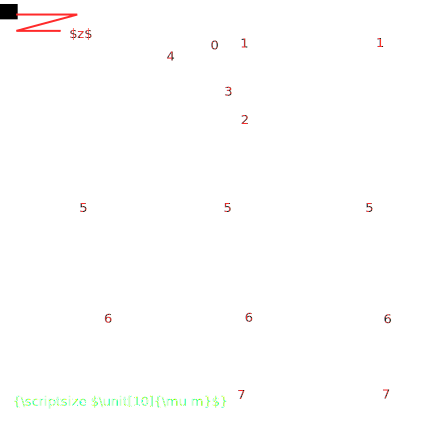
\includegraphics[width=12cm]{m_wf}
  \caption{Wide field stack of a three-dimensional distribution of
    yellow-green beads in agar. Sampling in $z$ is $\unit[1]{\mu m}$.}
  \label{fig:m_wf}
\end{figure}


\begin{figure}[hbtp]
  \centering
  \svginput{1}{m_sec}
  \caption{Computationally sectioned images. Note that two beads (4
    and 7) are very close to the border of the field of view and not
    fully illuminated.}
  \label{fig:m_sec}
\end{figure}


\begin{figure}[hbtp]
  \centering
  \svginput{1}{angular-beads}
  \caption{Spatio-angular controlled illumination of the beads from
    \figref{fig:m_sec}. The top left image shows bead number zero and
    so forth, the second image in the top shows bead number one and so
    on. The LCoS selectively illuminates the target bead and the MMA
    displays the pattern shown in \figref{fig:m_bfp_co}.}
  \label{fig:m_ang}
\end{figure}


\begin{figure}[!hbt]
  \centering
  \svginput{1}{montage-ang}
  \caption{}
  \label{fig:montage-ang}
\end{figure}




%%% Local Variables: 
%%% mode: latex
%%% TeX-master: "kielhorn_memi"
%%% End: 
